% SVN info for this file
\svnidlong
{$HeadURL$}
{$LastChangedDate$}
{$LastChangedRevision$}
{$LastChangedBy$}

\chapter{Varietà topologiche}
\labelChapter{varietà}

\begin{introduction}
	‘‘BEEP BOOP INSERIRE CITAZIONE QUA BEEP BOOP.''
	\begin{flushright}
		\textsc{NON UN ROBOT,} UN UMANO IN CARNE ED OSSA BEEP BOOP.
	\end{flushright}
\end{introduction}

\section{Varietà topologiche}
%AAA INTRODUZIONE BELLA CERCASI
Si vuole formalizzare il concetto di avere \textit{localmente} la topologia euclidea.
\begin{define}
	Uno spazio topologico $X$ si dice \textbf{localmente euclideo}\index{localmente euclideo} di dimensione $n$ se ogni punto di $X$ ammette un intorno aperto omeomorfo ad una palla aperta di $\realset^n$.
\end{define}

\begin{define}
	Uno spazio topologico $X$ si dice \textbf{varietà topologica}\index{varietà topologica} di dimensione $n$ se $X$ è $T_2$, connesso, a base numerabile e localmente euclideo di dimensione $n$.
\end{define}

\begin{examples}
	\begin{itemize}
		\item $\realset^n$ è una varietà topologica di dimensione $n$.
		\item $S^n$ è una varietà topologica compatta di dimensione $n$, infatti grazie alla proiezione stereografica si ha che $S^\setminus\{*\}\cong \realset$.
		\item $\mathbb{P}^n(\realset)$ è una varietà topologica compatta di dimensione $n$.
		\item Ogni aperto connesso di una varietà topologica di dimensione $n$ è una varietà topologica di dimensione $n$.
	\end{itemize}
\end{examples}
\begin{observe}
	La dimensione di una varietà topologica è \textit{ben definita} per l'\textit{invarianza} della dimensione.
\end{observe}
\begin{observe}
	\begin{itemize}
		\item Una varietà topologica è \textbf{c.p.a.}.
		\item Se $X$ è una varietà topologica di dimensione $n$ e $Y$ è una varietà topologica di dimensione $m$ allora $X\times Y$ è una varietà topologica di dimensione $n+m$.
	\end{itemize}
%DIMOSTRAZIONE TUTORATO dei due punti precedenti
\end{observe}
\begin{example}
	$T=S^1\times S^1$ è una varietà topologica di dimensione $2$.
\end{example}

\begin{theorema}
	Sia $X$ uno spazio topologico compatto, connesso, $T_2$ e localmente euclideo di dimensione $n$. Allora $X$ è a base numerabile, dunque $X$ è una varietà topologica di dimensione $n$.
\end{theorema}
 
	\subsection{Dimensione 1}
Analizziamo il caso di varietà topologiche di dimensione $1$, per esempio $\realset$ e $S^1$.
\begin{theorema}
	Ogni varietà topologica di dimensione $1$ è omeomorfo a $\realset$ se \textit{non} è compatta, oppure a $S^1$ se compatta.
\end{theorema} 
\begin{example} 
Riconsideriamo l'esempio della retta con 2 origini, vedasi la sezione \ref{retta 2 origini}, essa è un quoziente non $T_2$, dunque non è una varietà topologica.
\end{example}
	\subsection{Dimensione 2}
\begin{define} 
	Una varietà topologica di dimensione $2$ si dice \textbf{superficie topologica}\index{superficie!topologica}.
\end{define}
\begin{examples}
	\begin{itemize}
		\item $\realset^2$ o $\realset^2\setminus \{n \text{punti}\}$ sono \textit{non} compatti.
		\item $S^2$ compatto.
		\item $T=S^1\times S^1$ compatto.
		\item $\mathbb{P}^2(\realset)$ compatto.
	\end{itemize}
\end{examples}
Vogliamo dare una classificazione delle superfici topologiche \textit{compatte}. \footnote{Seguiremo le note del professore Gianluca Occhetta}
%BIBLIOGRAFIA
\begin{examples} \textsc{modelli piani}\\
	\begin{itemize}
		\item Siccome $\mathbb{P}^2(\realset)$ è un quoziente del disco, allora, a meno di omeomorfismo, lo si può anche vedere come un quoziente di $I\times I$ con una relazione di equivalenza sul bordo con \textit{parola} $abab$.
		\begin{center}
			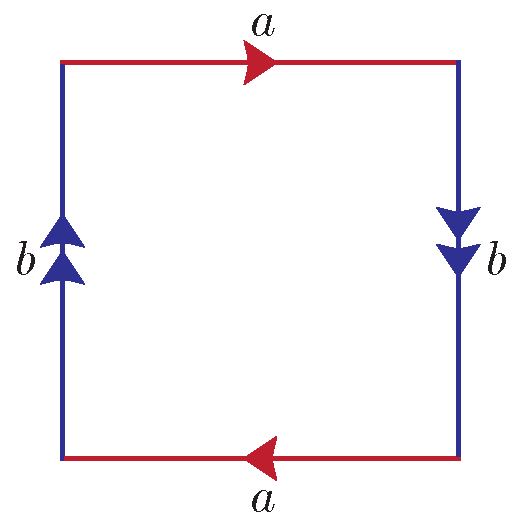
\includegraphics[trim=0cm 0cm 0cm 0cm, clip, scale=0.4]{images/proj.pdf}
		\end{center}
		\item Anche il \textbf{toro} si può vedere come quoziente di $I\times I$ con \textit{parola} $aba^{-1}b^{-1}$
		\begin{center}
			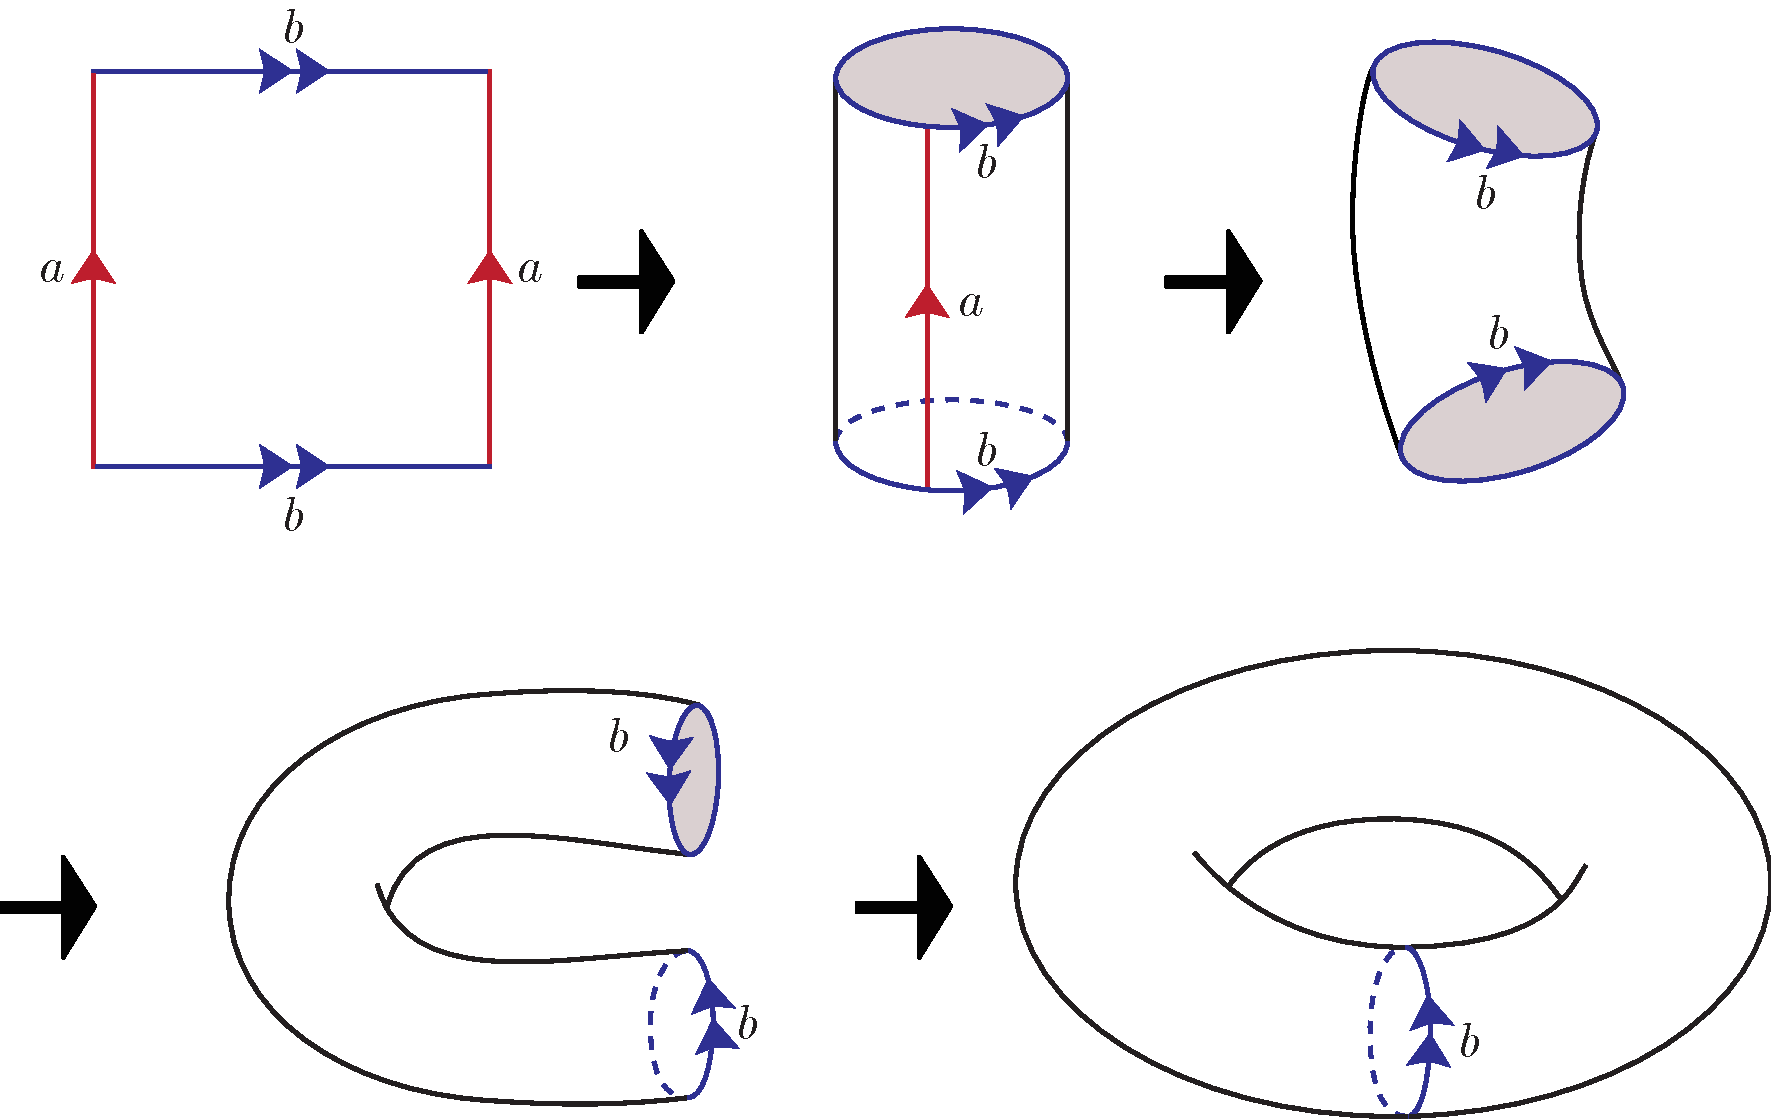
\includegraphics[trim=0cm 0cm 0cm 0cm, clip, scale=0.4]{images/torus.pdf}
		\end{center}
		\item Vediamo $S^2$ come quoziente di $I\times I$ con \textit{parola} $bb^{-1}a^{-1}a$.
		\begin{center}
			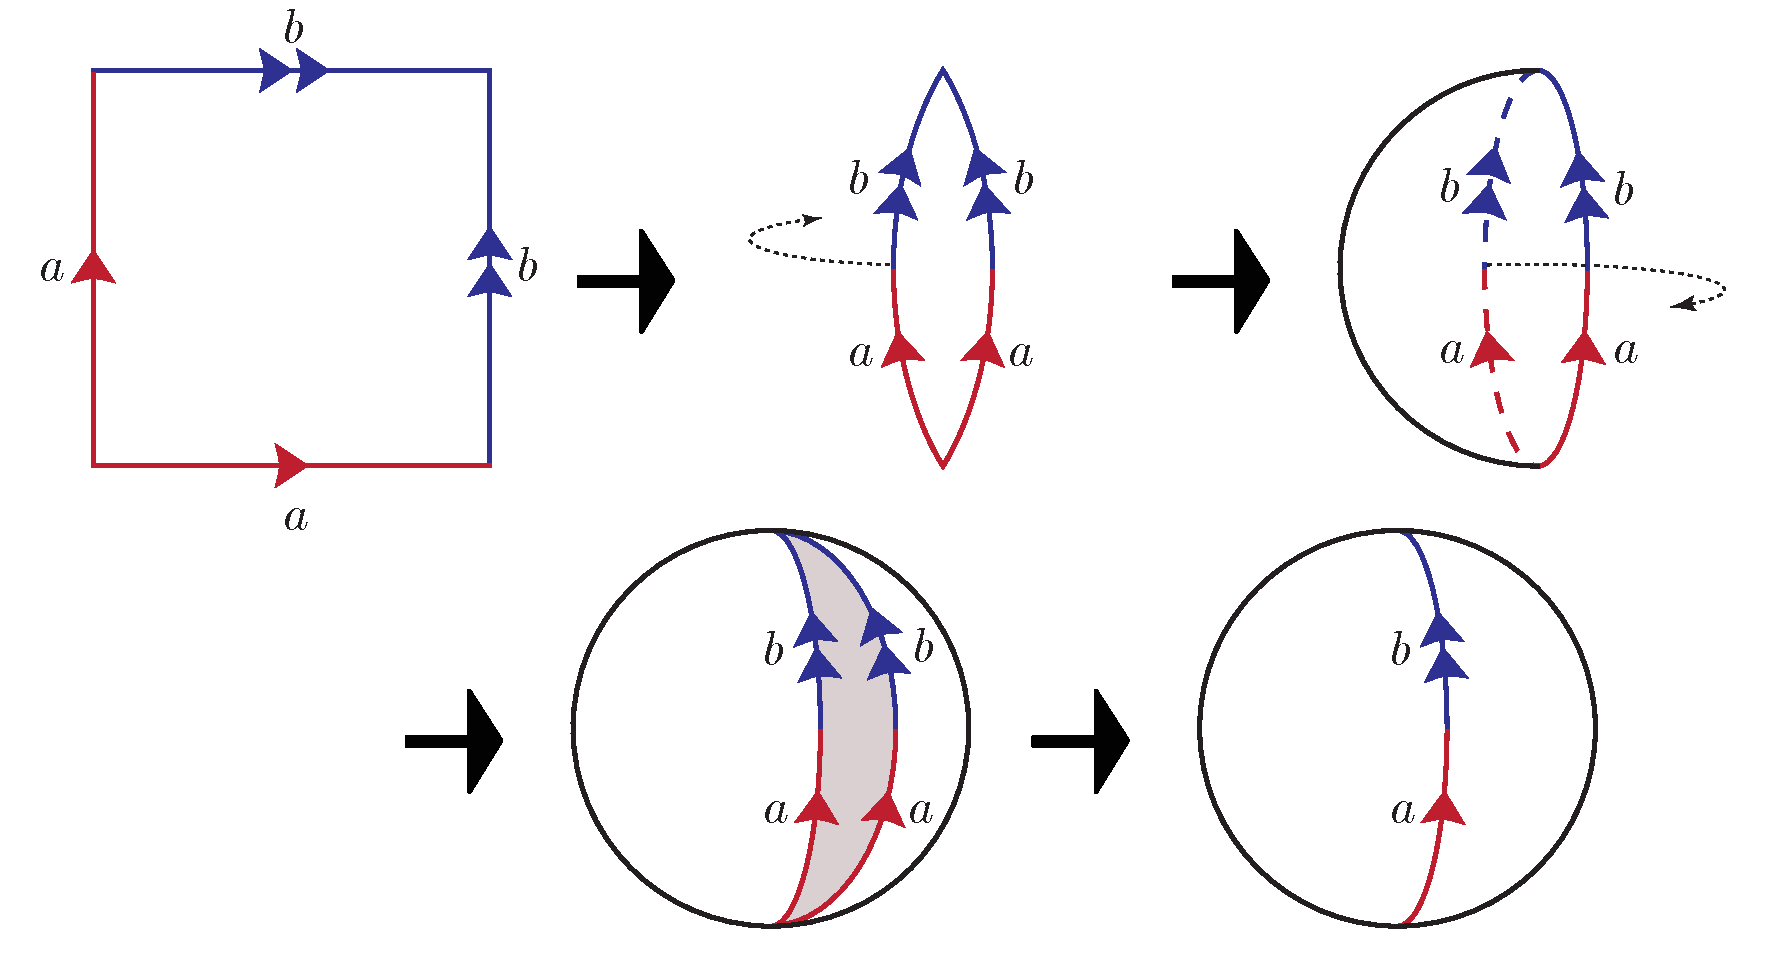
\includegraphics[trim=0cm 0cm 0cm 0cm, clip, scale=0.4]{images/sphere.pdf}
		\end{center}
	\end{itemize}
\end{examples}

\begin{observe}
	Sia $P\subset\realset^2$ un \textit{poligono} pieno con un numero pari di lati. Sia $\sim$ una relazione di equivalenza che identifica i lati a 2 a 2. Allora $S\coloneqq\nicefrac{P}{\sim}$ è una superficie topologica compatta, infatti:
		\begin{enumerate}
			\item  $P$ è connesso e compatto $\implies S$ connesso e compatto.
			\item $S$ è localmente euclideo di dimensione $2$. Sia $p\in S$, se $p$ viene da un punto interno al poligono allora si sceglie un intorno aperto $U$ centrato in tale punto tale che $U\cap\partial{P}=\emptyset$, data la proiezione $\funz \pi P S$, $\pi(U)\cong U$ ed è un intorno aperto di $p$. Se $p$ viene da un punto interno ad un lato grazie all'dentificazione dei lati a due a due si ha che passando al quoziente cìè un intorno aperto di $p$ omeomorfo ad un disco aperto. Se $p$ viene da un vertice, siccome i vertici vengono identificati con i vertici, analogamente al caso dei lati si ottiene un intorno aperto di $p$ in $S$ omeomorfo ad un disco aperto di $\realset^2$.
			\item $S$ è $T_2$.
		\end{enumerate}
	Osserviamo che nella relazione di equivalenza due lati vengono identificati nel modo seguente: $l_i\cong\intv$, dunque scelgo un omeomorfismo $l_1\stackrel{\stackrel{\phi}{\sim}}{\longrightarrow} l_2$, $p_1\in l_1 \sim \phi(p)\in l_2$ e $\phi$ manda vertici in vertici.\\
	Il poligono $P$ con la relazione di equivalenza sui lati è detto un \textbf{modello piano}\index{modello piano} della superficie $S$ e può essere schematizzato con una sequenza di lettere detta \textbf{parola}\index{parola}. Ad esempio, per la parola $aba^{-1}cbc^{-1}$ si ottiene il modello piano seguente:
	% https://q.uiver.app/?q=WzAsNixbMSwwLCJcXGJ1bGxldCJdLFsyLDAsIlxcYnVsbGV0Il0sWzMsMSwiXFxidWxsZXQiXSxbMCwxLCJcXGJ1bGxldCJdLFsxLDIsIlxcYnVsbGV0Il0sWzIsMiwiXFxidWxsZXQiXSxbMCwxLCJhIl0sWzEsMiwiYiJdLFswLDMsImMiLDJdLFs0LDMsImIiXSxbNSwyLCJhIiwyXSxbNSw0LCJjIl1d
	\[\begin{tikzcd}
		& {\bullet} & {\bullet} \\
		{\bullet} &&& {\bullet} \\
		& {\bullet} & {\bullet}
		\arrow["{a}", from=1-2, to=1-3]
		\arrow["{b}", from=1-3, to=2-4]
		\arrow["{c}"', from=1-2, to=2-1]
		\arrow["{b}", from=3-2, to=2-1]
		\arrow["{a}"', from=3-3, to=2-4]
		\arrow["{c}", from=3-3, to=3-2]
	\end{tikzcd}\]
 Inoltre il modello piano di una superficie compatta \textit{non è unico}.
\end{observe}



\begin{examples}
	\begin{itemize}
		\item $S^2$
		% https://q.uiver.app/?q=WzAsMixbMCwwLCJcXGJ1bGxldCJdLFswLDIsIlxcYnVsbGV0Il0sWzAsMSwiYSIsMix7ImN1cnZlIjozfV0sWzAsMSwiYSIsMCx7ImN1cnZlIjotM31dXQ==
		\[\begin{tikzcd}
			{\bullet} \\
			\\
			{\bullet}
			\arrow["{a}"', from=1-1, to=3-1, curve={height=18pt}]
			\arrow["{a}", from=1-1, to=3-1, curve={height=-18pt}]
		\end{tikzcd}\]
		\item $\mathbb{P}^2(\realset)$
		% https://q.uiver.app/?q=WzAsMixbMCwwLCJcXGJ1bGxldCJdLFswLDIsIlxcYnVsbGV0Il0sWzAsMSwiYSIsMix7ImN1cnZlIjozfV0sWzEsMCwiYSIsMix7ImN1cnZlIjozfV1d
		\[\begin{tikzcd}
			{\bullet} \\
			\\
			{\bullet}
			\arrow["{a}"', from=1-1, to=3-1, curve={height=18pt}]
			\arrow["{a}"', from=3-1, to=1-1, curve={height=18pt}]
		\end{tikzcd}\]
		\item La Bottiglia di Klein $K$, essa è la superficie compatta data dal modello piano. Confrontiamolo con il toro. Incolliamo entrambi i modelli: prima si ottiene $S^1\times I$ con la relazione di equivalenza sul bordo.
		% https://q.uiver.app/?q=WzAsMTYsWzAsNCwiXFxidWxsZXQiXSxbMCw2LCJcXGJ1bGxldCJdLFsyLDQsIlxcYnVsbGV0Il0sWzIsNiwiXFxidWxsZXQiXSxbNSw0LCJcXGJ1bGxldCJdLFs3LDQsIlxcYnVsbGV0Il0sWzUsNiwiXFxidWxsZXQiXSxbNyw2LCJcXGJ1bGxldCJdLFswLDIsIlxcYnVsbGV0Il0sWzAsMCwiXFxidWxsZXQiXSxbMiwwLCJcXGJ1bGxldCJdLFsyLDIsIlxcYnVsbGV0Il0sWzUsMiwiXFxidWxsZXQiXSxbNSwwLCJcXGJ1bGxldCJdLFs3LDAsIlxcYnVsbGV0Il0sWzcsMiwiXFxidWxsZXQiXSxbMCwxLCIiLDIseyJzdHlsZSI6eyJoZWFkIjp7Im5hbWUiOiJub25lIn19fV0sWzIsMywiIiwyLHsic3R5bGUiOnsiaGVhZCI6eyJuYW1lIjoibm9uZSJ9fX1dLFswLDIsImIiLDIseyJjdXJ2ZSI6Mn1dLFswLDIsIiIsMSx7ImN1cnZlIjotMiwic3R5bGUiOnsiaGVhZCI6eyJuYW1lIjoibm9uZSJ9fX1dLFszLDEsImIiLDAseyJjdXJ2ZSI6LTJ9XSxbMSwzLCIiLDAseyJjdXJ2ZSI6LTIsInN0eWxlIjp7ImJvZHkiOnsibmFtZSI6ImRvdHRlZCJ9LCJoZWFkIjp7Im5hbWUiOiJub25lIn19fV0sWzQsNSwiYiIsMix7ImN1cnZlIjoyfV0sWzQsNSwiIiwwLHsiY3VydmUiOi0yLCJzdHlsZSI6eyJoZWFkIjp7Im5hbWUiOiJub25lIn19fV0sWzYsNywiYiIsMix7ImN1cnZlIjoyfV0sWzYsNywiIiwwLHsiY3VydmUiOi0yLCJzdHlsZSI6eyJib2R5Ijp7Im5hbWUiOiJkb3R0ZWQifSwiaGVhZCI6eyJuYW1lIjoibm9uZSJ9fX1dLFs0LDYsIiIsMSx7InN0eWxlIjp7ImhlYWQiOnsibmFtZSI6Im5vbmUifX19XSxbNSw3LCIiLDEseyJzdHlsZSI6eyJoZWFkIjp7Im5hbWUiOiJub25lIn19fV0sWzgsOSwiYSJdLFs5LDEwLCJiIl0sWzExLDEwLCJhIiwyXSxbMTEsOCwiYiJdLFsxMiwxMywiYSJdLFsxMywxNCwiYiJdLFsxMiwxNSwiYiIsMl0sWzE1LDE0LCJhIiwyXV0=
		\[\begin{tikzcd}
			{\bullet} && {\bullet} &&& {\bullet} && {\bullet} \\
			\\
			{\bullet} && {\bullet} &&& {\bullet} && {\bullet} \\
			\\
			{\bullet} && {\bullet} &&& {\bullet} && {\bullet} \\
			\\
			{\bullet} && {\bullet} &&& {\bullet} && {\bullet}
			\arrow[from=5-1, to=7-1, no head]
			\arrow[from=5-3, to=7-3, no head]
			\arrow["{b}"', from=5-1, to=5-3, curve={height=12pt}]
			\arrow[from=5-1, to=5-3, curve={height=-12pt}, no head]
			\arrow["{b}", from=7-3, to=7-1, curve={height=-12pt}]
			\arrow[from=7-1, to=7-3, curve={height=-12pt}, dotted, no head]
			\arrow["{b}"', from=5-6, to=5-8, curve={height=12pt}]
			\arrow[from=5-6, to=5-8, curve={height=-12pt}, no head]
			\arrow["{b}"', from=7-6, to=7-8, curve={height=12pt}]
			\arrow[from=7-6, to=7-8, curve={height=-12pt}, dotted, no head]
			\arrow[from=5-6, to=7-6, no head]
			\arrow[from=5-8, to=7-8, no head]
			\arrow["{a}", from=3-1, to=1-1]
			\arrow["{b}", from=1-1, to=1-3]
			\arrow["{a}"', from=3-3, to=1-3]
			\arrow["{b}", from=3-3, to=3-1]
			\arrow["{a}", from=3-6, to=1-6]
			\arrow["{b}", from=1-6, to=1-8]
			\arrow["{b}"', from=3-6, to=3-8]
			\arrow["{a}"', from=3-8, to=1-8]
		\end{tikzcd}\]
	\end{itemize}
\end{examples}

	\subsection{Somma connessa}
Siano $S_1$ e $S_2$ superfici compatte e siano $x\in S_1$ e $y\in S_2$. Siano $D_x\subset S_1$ e $D_y\subset S_2$ intorni di $x$ e $y$ rispettivamente, omeomorfi ad un disco chiuso $D\subset\realset^2$, dunque $D_x\stackrel{\stackrel{h}{\sim}}{\longrightarrow} D_y$. Togliamo dalle due superfici gli intorni dei dischetti, sia $Y\coloneqq (S_1\setminus \interior{D_x})\amalg (S_2\setminus \interior{D_y})$, incolliamo i due pezzi di $Y$ lungo i bordi dei dischi, cioé mettiamo su $Y$ la relazione di equivalenza $x_1\sim y_1 \iff x_1=y_1$ oppure $x_1\in\partial{D},\ y_1\in\partial{D}$ e $y_1=h(x_1)$ o viceversa.\newline
Vediamo ora qualche fatto che non dimostriamo:
	\begin{itemize}
		\item il quoziente è ancora una superficie topologica, che denotiamo con $S_1\# S_2$ \textbf{somma connessa} di $S_1$ e $S_2$
		\item la somma connessa $S_1\# S_2$ a meno di omeomorfismo non dipende dalle scelte fatte come i punti $x$ e $y$, gli intorni $D_x$ e $D_y$, l'omeomorfismo $h$, ma soltanto da $S_1$ e da $S_2$!
	\end{itemize}



